\documentclass[11pt,a4paper]{article}
\usepackage[utf8]{inputenc}
\usepackage[T1]{fontenc}
\usepackage{lmodern}
\usepackage{graphicx}
\usepackage{amsmath,amssymb}
\usepackage{booktabs}
\usepackage{array}
\usepackage{geometry}
\usepackage{microtype}
\usepackage[font=small,labelfont=bf]{caption}
\usepackage[colorlinks=true,citecolor=blue,linkcolor=blue,urlcolor=blue]{hyperref}
\geometry{margin=2.4cm}
\graphicspath{{figures/}{.}}

\renewcommand{\topfraction}{0.90}
\renewcommand{\bottomfraction}{0.70}
\renewcommand{\textfraction}{0.08}
\renewcommand{\floatpagefraction}{0.80}

\newcommand{\avg}[1]{\langle #1\rangle}
\newcommand{\Dbar}{\overline{D}}
\newcommand{\Eact}{E_{\mathrm{act}}}
\newcommand{\Plid}{P_{\mathrm{lid}}}
\newcommand{\Sij}{\mathbf{S}}

\title{\bfseries Spatio-temporal wall-actuation modes and cycle-mean\\
viscous dissipation in a lid-driven cavity}

\author{Beniaiche Ahmed$^{1,}$\thanks{Corresponding author: beniaiche\_ahmed25@yahoo.fr}, Larabi Abderrahim$^{1}$, Belkadi Mbarek$^{2}$\\[4pt]
$^{1}$Laboratory of Fluid Mechanics, Ecole Militaire Polytechnique, Algiers, Algeria\\
$^{2}$Laboratory of Turbomachinery, Ecole Militaire Polytechnique, Algiers, Algeria}
\date{}

\begin{document}
\maketitle

\begin{abstract}
The spatial and temporal organization of wall actuation determines how mechanical
input is distributed across the flow structures of a driven cavity, yet the
resulting viscous-dissipation cost cannot be inferred from the actuation spectrum
or from the time-mean velocity field alone. This study examines the relationship
between wall-actuation structure, hydrodynamic response, and cycle-mean viscous
dissipation in a two-dimensional lid-driven cavity. Stationary harmonic profiles
and three physics-informed actuation branches are transferred to an independent
multiple-relaxation-time lattice-Boltzmann solver and compared at a common
quadratic actuation norm. For stationary controls at $Re=500$, the first spatial
harmonic reduces dissipation by $17.7\%$ relative to a corner-regularized
uniform-lid reference, whereas the second harmonic and the mean profile of the
second-mode-dominated branch increase it by $36.8\%$ and $44.3\%$, respectively.
Grid-refinement and local strain-rate analyses associate this ordering with the
redistribution of dissipation between corner shear layers and the cavity interior.
For time-dependent branches, the cycle-mean dissipation differs markedly from the
dissipation of the time-mean flow. In particular, the temporally dominated branch
has a cycle-mean dissipation approximately $3.1$ times that of the predominantly
stationary branch, despite its much weaker mean-flow contribution. The results
demonstrate that the energetic cost of wall actuation depends on both the spatial
organization and the temporal fluctuations of the resulting flow, and that physical
performance must be assessed using cycle-averaged dissipation rather than modal
accessibility or mean-field diagnostics alone.
\end{abstract}

\noindent\textbf{Keywords:} lid-driven cavity; wall actuation; viscous dissipation;
energy budget; mean-flow diagnostics; mode selection

%----------------------------------------------------------------------
\section*{Nomenclature}
%----------------------------------------------------------------------

\begin{center}
\footnotesize
\renewcommand{\arraystretch}{1.0}
\setlength{\tabcolsep}{2.5pt}
\begin{tabular}{@{}l>{\raggedright\arraybackslash}p{0.78\textwidth}@{}}
\toprule
\multicolumn{2}{@{}l}{\textit{Roman symbols}}\\
\midrule
\(A_\varepsilon\) & half-spread of \(D(t)\) over the cycle, i.e.\ the variability concealed by a single cycle-mean number\\
\(AR\) & cavity aspect ratio, \(L_x/L_y\)\\
\(C_3\) & spectral rank concentration, sum of the three largest control-energy fractions\\
\(D\) & instantaneous viscous dissipation rate, \((2/Re)\int_\Omega \mathbf{S}\!:\!\mathbf{S}\,d\Omega\)\\
\(\Dbar\) & cycle-mean dissipation, \(\langle D\rangle_t\)\\
\(E_{\mathrm{act}}\) & instantaneous actuation energy of the lid profile, \(\int_0^1 U_{\mathrm{lid}}^2\,dx\)\\
\(E_r\) & realized cycle-averaged actuation energy of a transferred control\\
\(E^*\) & prescribed target actuation energy\\
\(f_1,f_2,f_t\) & first-harmonic, second-harmonic, and explicitly time-dependent control-energy fractions\\
\(H_N\) & normalized branch-selection entropy\\
\(K\) & kinetic energy, \(\tfrac12\int_\Omega |\mathbf{u}|^2\,d\Omega\)\\
\(L,L_x,L_y\) & cavity side, streamwise and wall-normal lengths\\
\(N\) & number of lattice nodes per cavity side (LBM resolution)\\
\(P_{\mathrm{lid}}\) & mechanical power injected through the lid, \(\int_0^1 U_{\mathrm{lid}}\tau_w\,dx\)\\
\(R_K\) & ratio of fluctuating to mean kinetic energy\\
\(Re\) & Reynolds number, \(U_{\mathrm{ref}}L/\nu\)\\
\(\mathbf{S}\) & strain-rate tensor, \((\nabla\mathbf{u}+\nabla\mathbf{u}^{\mathsf T})/2\)\\
\(t,T\) & time and forcing period\\
\(\mathbf{u}=(u,v)\) & velocity vector and its streamwise/wall-normal components\\
\(u'\) & fluctuating velocity, \(\mathbf{u}-\langle\mathbf{u}\rangle\)\\
\(u'_{\mathrm{rms}}\) & root-mean-square temporal fluctuation at a fixed point\\
\(U_{\mathrm{lid}}\) & lid velocity profile (the actuation)\\
\(U_{\mathrm{ref}}\) & reference velocity, the amplitude of the uniform lid\\
\(x,y\) & streamwise and wall-normal coordinates\\
\midrule
\multicolumn{2}{@{}l}{\textit{Greek symbols and branch symbols}}\\
\midrule
\(B_1,B_2,B_3\) & empirical branch classes (second-harmonic dominated, time-dependent dominated, residual)\\
\(B_{\mathrm{first}}\) & first-harmonic branch class of the full-spectrum audit\\
\(\delta\) & corner taper width\\
\(\varepsilon\) & integrated viscous dissipation accumulated over an LBM sampling window\\
\(\lambda_{\mathrm{var}}\) & weight of the variance-regularization term of the training loss\\
\(\nu\) & kinematic viscosity\\
\(\tau_w\) & wall shear stress on the moving lid\\
\(\psi\) & stream function\\
\(\Omega\) & cavity domain\\
\midrule
\multicolumn{2}{@{}l}{\textit{Abbreviations}}\\
\midrule
GCI & grid-convergence index\\
LBM & lattice-Boltzmann method\\
LOCO & leave-one-Reynolds-condition-out (cross-validation)\\
MRT & multiple-relaxation-time\\
PINN & physics-informed neural network\\
RMSE & root-mean-square error\\
\bottomrule
\end{tabular}
\end{center}

%----------------------------------------------------------------------
\section{Introduction}
%----------------------------------------------------------------------

Wall actuation is one of the few ways in which the vortical structure of a
confined recirculating flow can be modified without changing its geometry. In a
lid-driven cavity the entire vortex topology is generated by the tangential
motion of a single boundary, so any spatial structure imposed on that boundary
acts directly on the mechanism that sustains the flow. The cavity is therefore a
natural configuration in which to ask a question that is central to flow control
but rarely posed in energetic terms: when two different actuations require the
same control effort, which one produces the less dissipative flow, and why?
The canonical cavity solution and its benchmarks are well established
\cite{ghia1982high,botella1998benchmark,shankardeshpande2000,albensoeder2005accurate,kuhlmann2019},
and the flow has long served as a test bed for control strategies
\cite{gadelhak2000,brunton2015closed}, yet its dissipation budget under
distributed wall actuation has received comparatively little attention.

The energetic mechanism is twofold, and the two parts can act in opposite
directions. Changing the wall velocity changes the mechanical power injected into
the fluid,
$\Plid=\int_0^1 U_{\mathrm{lid}}\tau_w\,dx$, where $\tau_w$ is the wall shear
stress; it also changes the spatial distribution of the strain-rate tensor
$\Sij$, and with it the partition of viscous dissipation between the lid shear
layer, the side-wall layers, the cavity interior and the two upper corners, where
a discontinuous lid produces a stress singularity. A profile can therefore reduce
the peak strain at the corners while increasing the strain everywhere else, and
the net effect is not predictable from the shape of the actuation alone. The
distinction matters because the two natural comparison protocols answer different
questions. Comparing profiles at the same lid-velocity scale
\cite{beniaiche2026} measures what a given actuator amplitude achieves; comparing
them at the same quadratic actuation norm
$\Eact=\int_0^1U_{\mathrm{lid}}^2\,dx$ measures what a given control effort
achieves. The two rankings need not agree, and only the second is a statement
about the energetic response at fixed actuation norm. A further distinction, specific to time-dependent actuation, is
that the dissipation of the time-mean field is not the time mean of the
instantaneous dissipation: because $D$ is quadratic in the velocity gradients,
cycle-averaged dissipation always exceeds the dissipation of the mean flow, and
the gap can be orders of magnitude when the fluctuations dominate
\cite{pope2000,landau1987}.

Spatially structured and time-periodic actuations can also support more than one
hydrodynamic response. A periodic boundary-value problem of this type admits
several coexisting branches, and which one is reached depends on the formulation,
the regularization and the initialization of the identification procedure. A
preceding study by Beniaiche \cite{beniaiche2026} investigated the identification
and independent numerical verification of conditional modal collapse in
physics-informed active control of the lid-driven cavity. It established that the
identified actuation is not characterized by a unique, universally selected modal
structure: predominantly stationary second-harmonic controls and strongly
time-dependent alternatives can be recovered depending on initialization,
regularization, and control parameterization. Independent MRT-LBM simulations
further demonstrated that these identified controls can produce physically
distinct cavity responses. The emphasis of that work was on branch identification,
conditional accessibility, and independent numerical reproducibility. The present
study addresses the complementary fluid-mechanical question of how these spatial
and temporal actuation structures affect the viscous-dissipation budget of the
resulting flow. Rather than treating modal recovery as a performance criterion, we
quantify the dissipation of stationary and periodic responses under a common
quadratic actuation norm, distinguish the dissipation of the time-mean field from
the cycle-mean dissipation, and identify the strain-rate distributions responsible
for the observed energetic differences.

The question addressed in this paper is accordingly:
\begin{quote}
How does the spatio-temporal structure of wall actuation determine the cycle-mean
viscous dissipation of the resulting cavity flow at a prescribed
actuation-energy level?
\end{quote}
The sequence of the paper follows that question. Section~\ref{sec:formulation}
fixes the physical and energetic framework, and in particular separates the
quadratic actuation norm from the mechanical power transmitted through the wall.
Section~\ref{sec:modes} defines the stationary modes and the three identified
branches that are compared. Section~\ref{sec:methods} describes how the
actuations are identified and how the flows are computed independently.
Section~\ref{sec:stationary} reports the energetic response of the stationary
modes, Section~\ref{sec:branches_results} the cycle-mean response of the time-dependent
branches, and Section~\ref{sec:interpretation} interprets both in terms of local
strain and fluctuating gradients. Section~\ref{sec:conclusions} concludes.

%----------------------------------------------------------------------
\section{Physical formulation and energetic framework}
\label{sec:formulation}
%----------------------------------------------------------------------

\subsection{Controlled cavity and governing equations}

We consider a two-dimensional incompressible flow in the square cavity
$0\le x\le 1$, $0\le y\le 1$, made dimensionless with the cavity height $L$ and a
reference velocity $U_0$ (Fig.~\ref{fig:modes}a). The lower and lateral walls are no-slip and stationary;
the upper wall moves tangentially with a velocity profile
$U_{\mathrm{lid}}(x,t)$ that is the control variable. The velocity field
$\mathbf{u}=(u,v)$ and the pressure $p$ satisfy
\begin{equation}
\frac{\partial\mathbf{u}}{\partial t}+(\mathbf{u}\cdot\nabla)\mathbf{u}
=-\nabla p+\frac{1}{Re}\nabla^{2}\mathbf{u},
\qquad \nabla\cdot\mathbf{u}=0,
\label{eq:ns}
\end{equation}
with $Re=U_0L/\nu$, subject to
\begin{equation}
\mathbf{u}=\mathbf{0}\ \ \text{on } x=0,\,x=1,\,y=0,
\qquad
u=U_{\mathrm{lid}}(x,t),\ \ v=0\ \ \text{on } y=1 .
\label{eq:bc}
\end{equation}
A pointwise tangential velocity along the lid idealizes an array of independently
driven wall segments, or a distributed momentum source such as a
dielectric-barrier-discharge actuator, whose near-wall forcing is equivalent in
the time-averaged sense used here to a tangential wall velocity
\cite{corke2010dbd}. Because $U_0$ is a scaling velocity and not a property of
the lid, a profile may change sign along $x$ or in time; the amplitude of the
actuation is fixed separately by the norm constraint introduced in
Sec.~\ref{sec:norm}.

\subsection{The quadratic actuation norm and the mechanical wall power}
\label{sec:norm}

Two different scalar quantities characterize a wall actuation, and they must not
be conflated. The first is the \emph{quadratic actuation norm}
\begin{equation}
\Eact(t)=\int_0^1 U_{\mathrm{lid}}^2(x,t)\,dx,
\qquad
\overline{E}_{\mathrm{act}}=\frac{1}{T}\int_0^T\Eact(t)\,dt,
\label{eq:eact}
\end{equation}
which measures the squared amplitude of the commanded wall velocity, has units of
$U_0^2L$, and is the quantity held fixed in all comparisons below. It is a norm of
the boundary data, not a work: it contains no information about the fluid response.
The second is the \emph{mechanical power} transmitted by the lid,
\begin{equation}
\Plid(t)=\int_0^1 U_{\mathrm{lid}}(x,t)\,\tau_w(x,t)\,dx,
\qquad
\tau_w=\frac{1}{Re}\left.\frac{\partial u}{\partial y}\right|_{y=1},
\label{eq:plid}
\end{equation}
positive when the wall does work on the fluid. $\Plid$ depends on the actuation
and on the flow through the wall shear stress, and it is the quantity that enters
the energy balance. Two actuations of equal $\overline{E}_{\mathrm{act}}$ can
therefore inject very different amounts of power; conversely, a large norm does
not guarantee a large power if the wall shear is weak.

Holding $\overline{E}_{\mathrm{act}}$ fixed also fixes the root-mean-square wall
velocity, $\overline{E}_{\mathrm{act}}^{1/2}=0.5$ at the value $E^\ast=0.25$ used
throughout, but not the maximum wall velocity. A uniform lid of unit shape then
has amplitude $0.5$, whereas a first harmonic of the same norm has amplitude
$\sqrt{2E^\ast}=0.7071$; a peakier profile has a larger maximum still. Because
the viscosity is fixed, a profile whose peak wall velocity is $U_{\max}$ realizes
an effective Reynolds number $Re_{\max}=U_{\max}Re$ based on that peak. The
comparisons below are therefore comparisons at equal quadratic actuation norm, at
fixed viscosity and geometry, and \emph{not} at equal $Re_{\max}$; the values of
$U_{\max}$ and $Re_{\max}$ are tabulated for every case
(Tables~\ref{tab:modes} and~\ref{tab:stationary}) so that the distinction is
explicit at every step. This convention differs from the fixed-lid-velocity
comparison of Ref.~\cite{beniaiche2026}, in which the peak velocity was the same
for all profiles and the norm differed by up to a factor of four.

\subsection{Viscous dissipation and its cycle mean}

For an incompressible Newtonian fluid the instantaneous viscous dissipation rate is
\begin{equation}
D(t)=\frac{2}{Re}\int_\Omega \Sij:\Sij\,d\Omega,
\qquad
\Sij=\tfrac12\left(\nabla\mathbf{u}+\nabla\mathbf{u}^{T}\right),
\label{eq:diss}
\end{equation}
and the quantity relevant to a periodic actuation is its cycle average
\begin{equation}
\Dbar=\frac{1}{T}\int_0^T D(t)\,dt .
\label{eq:dbar}
\end{equation}
Splitting the velocity into a time mean and a fluctuation,
$\mathbf{u}=\overline{\mathbf{u}}+\mathbf{u}'$ with
$\Sij=\overline{\Sij}+\Sij'$, the cycle mean decomposes exactly as
\begin{equation}
\Dbar
= \underbrace{\frac{2}{Re}\int_\Omega \overline{\Sij}:\overline{\Sij}\,d\Omega}
_{D(\overline{\mathbf{u}})}
+ \underbrace{\frac{2}{Re}\left\langle\int_\Omega \Sij':\Sij'\,d\Omega\right\rangle}_{\text{fluctuating part}},
\label{eq:jensen}
\end{equation}
because the cross term vanishes upon averaging. The two terms coincide only in the
steady limit; otherwise $\Dbar>D(\overline{\mathbf{u}})$, with a gap that measures
how much of the dissipation is carried by the unsteady part of the response.
Evaluating $D$ on a time-averaged field is thus not an approximation of
$\Dbar$ with a small error: it is a different functional, and for a strongly
unsteady flow it can invert the ranking of two actuations.

\subsection{Mechanical energy budget}

With the kinetic energy $K=\tfrac12\int_\Omega|\mathbf{u}|^2\,d\Omega$, the
momentum equation gives
\begin{equation}
\frac{dK}{dt}=\Plid(t)-D(t).
\label{eq:budget}
\end{equation}
For a periodic state the left-hand side integrates to zero over one period, so
\begin{equation}
\boxed{\ \overline{P}_{\mathrm{lid}}=\Dbar\ }
\label{eq:closure}
\end{equation}
is an exact identity of the governing equations. In the numerical evaluation of
Eq.~\eqref{eq:closure} both terms are computed from the same discrete fields, but
$\Plid$ involves a wall-normal derivative at the boundary, which is evaluated with
a one-sided finite difference and therefore carries a truncation error that $D$
does not. The budget is used below as a verification of the transfer and of the
periodicity of the response, with that estimator uncertainty made explicit
(Sec.~\ref{sec:budget}); it is not used as an exact closure constraint.

%----------------------------------------------------------------------
\section{Actuation modes and hydrodynamic states}
\label{sec:modes}
%----------------------------------------------------------------------

\subsection{Stationary reference profiles}

Five stationary profiles define the comparison, all normalized to
$E^\ast=0.25$. The \emph{uniform} lid $U_{\mathrm{lid}}=0.5$ is the reference of
the problem statement; it carries a tangential-velocity discontinuity at the two
upper corners, which is retained because it is the classical boundary condition,
but which is shown in Sec.~\ref{sec:corner} to prevent the convergence of its own
dissipation. A \emph{corner-regularized uniform} lid, constructed with an initial
plateau $U_p=0.5$ and a raised-cosine taper of width $\delta=0.05$ at each corner
\begin{equation}
U_{\mathrm{lid}}^{\mathrm{raw}}(x)=
\begin{cases}
\displaystyle
\frac{U_p}{2}
\left[1-\cos\!\left(\frac{\pi x}{\delta}\right)\right],
& 0\leq x<\delta,\\[6pt]
U_p,
& \delta\leq x\leq 1-\delta,\\[6pt]
\displaystyle
\frac{U_p}{2}
\left[1-\cos\!\left(\frac{\pi(1-x)}{\delta}\right)\right],
& 1-\delta<x\leq 1,
\end{cases}
\label{eq:taper}
\end{equation}
then rescaled to the prescribed norm:
\begin{equation}
U_{\mathrm{lid}}(x)=c\,U_{\mathrm{lid}}^{\mathrm{raw}}(x),
\qquad
c=
\sqrt{
\frac{E^\ast}
{\displaystyle\int_0^1
\left(U_{\mathrm{lid}}^{\mathrm{raw}}\right)^2 dx}
}.
\end{equation}
For $\delta=0.05$, the raw profile carries $E_{\mathrm{raw}}/E_{\mathrm{uniform}}
=1-5\delta/4=0.9375$, a $6.25\%$ loss which is restored by the rescaling factor
$c=\sqrt{16/15}\approx 1.033$; the final plateau value is approximately $0.5164$,
corresponding to $U_{\max}=0.52$ in table~\ref{tab:modes}. This regularized
profile removes the discontinuity and provides a converged reference. The first and second spatial harmonics,
$U_{\mathrm{lid}}=\sqrt{2E^\ast}\sin(\pi x)$ and
$\sqrt{2E^\ast}\sin(2\pi x)$, are the two elementary spatially structured
controls. Finally, the time-mean profile of the identified $B_1$ branch
(Sec.~\ref{sec:branches}) is included as the stationary approximation of a
physics-informed control.

\begin{figure}[t]
\centering
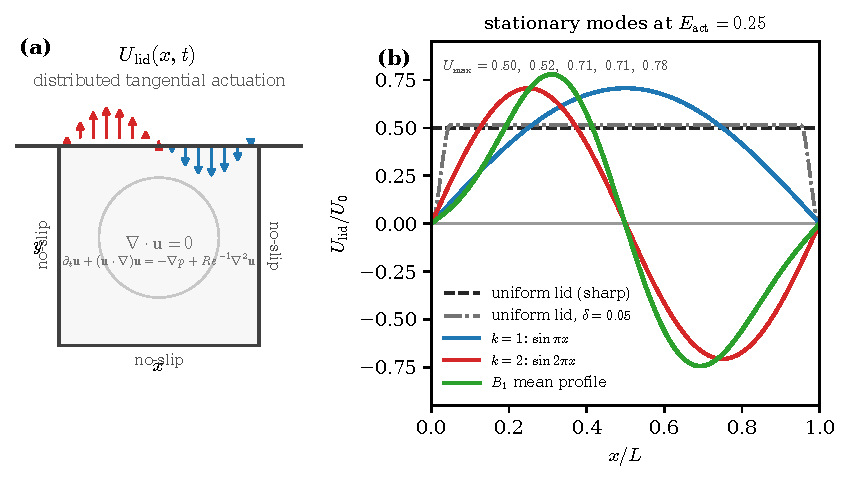
\includegraphics[width=\textwidth]{figures/fig01_modes.pdf}
\caption{(a) Geometry of the controlled cavity. The upper wall moves tangentially
with a distributed profile $U_{\mathrm{lid}}(x,t)$; the three other walls are
no-slip and stationary. (b) The five stationary actuation profiles compared in
this study, all normalized to the same quadratic actuation norm
$E^\ast=\int_0^1U_{\mathrm{lid}}^2\,dx=0.25$. The maximum wall velocity differs
between profiles at equal norm: $U_{\max}=0.50$ for the uniform lid, $0.71$ for
the two harmonics and $0.78$ for the $B_1$ mean profile.}
\label{fig:modes}
\end{figure}

\subsection{Identified actuation branches}
\label{sec:branches}

The time-dependent actuations are three representatives identified by the
physics-informed procedure of Sec.~\ref{sec:methods} and classified by the modal
energy of their control coefficients (details of the identification campaign and
classification rules are provided in Supplementary Secs.~S1--S3, particularly
Sec.~S2.3, Tables~S2--S3 and Fig.~S1). Writing the lid as
\begin{equation}
U_{\mathrm{lid}}(x,t)=\sum_{m=1}^{N_x}\sum_{n=0}^{N_t-1}
a_{mn}\sin(m\pi x)\cos\!\left(\frac{2n\pi t}{T}\right),
\label{eq:fourier}
\end{equation}
with forcing period \(T=2\),
the energy of coefficient $(m,n)$ is $\mathcal{E}_{m0}=\tfrac12a_{m0}^2$ and
$\mathcal{E}_{mn}=\tfrac14a_{mn}^2$ for $n\ge1$, with normalized fractions
$f_{mn}=\mathcal{E}_{mn}/\sum\mathcal{E}_{ij}$. The stationary second-harmonic
fraction is $f_2\equiv f_{20}$ and the total time-dependent fraction is
$f_t=\sum_{m=1}^{N_x}\sum_{n=1}^{N_t-1}f_{mn}$. The three classes are defined by modal dominance
\cite{beniaiche2026}: $B_1$ has $f_2>2f_t$ and $f_2>0.5$ (stationary
second-harmonic dominated); $B_2$ has $f_t>2f_2$ and $f_t>0.5$ (temporally
dominated); $B_3$ satisfies neither condition (mixed). At $Re=500$ and
$E^\ast=0.25$ the representatives used here have
$(f_2,f_t)=(0.93,0.07)$ for $B_1$, $(0.00,1.00)$ for $B_2$ (seed 5) and
$(0.52,0.45)$ for $B_3$ (seed 0), with a first-harmonic content
$f_1=0.006$ for $B_3$ and below $0.02$ for the other two.

The $B_1$ representative is used in two forms. The \emph{full} series is the
control as identified, including its small temporal content; the \emph{mean
profile} is its time average, a stationary actuation that isolates the spatial
structure. The stationary comparison of Sec.~\ref{sec:stationary} uses the mean
profile and the cycle-mean comparison of Sec.~\ref{sec:branch_compare} uses the full
series, so that the effect of the spatial structure is never conflated with the
effect of the temporal one. Representative profiles and their space--time
structure are shown in Fig.~\ref{fig:signatures}; Table~\ref{tab:modes}
collects the characteristics of the eight primary actuation cases compared in the paper.

\begin{figure}[t]
\centering
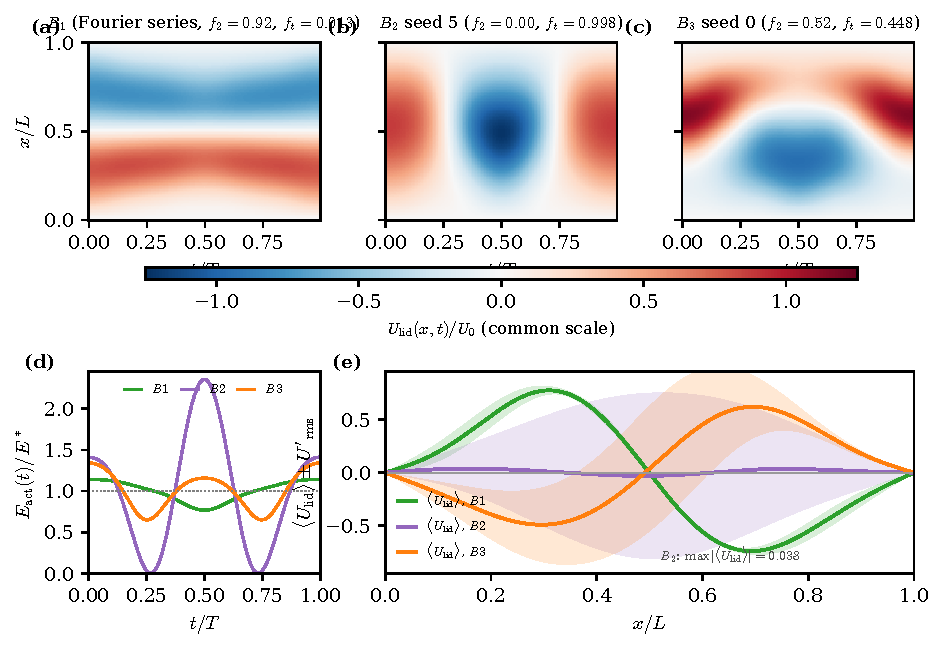
\includegraphics[width=\textwidth]{figures/fig02_signatures.pdf}
\caption{Spatio-temporal structure of the three identified branch controls at
$Re=500$ and $\overline{E}_{\mathrm{act}}=0.25$. (a)--(c) Lid velocity
$U_{\mathrm{lid}}(x,t)$ over one forcing period, on a common colour scale.
$B_1$ is nearly stationary; $B_2$ oscillates with a full sign reversal, the wall
velocity vanishing twice per period; $B_3$ combines a stationary two-lobe pattern
with a strong oscillation. (d) Instantaneous actuation norm $\Eact(t)$ normalized
by the common cycle-mean target: $B_2$ spans $0.004$--$2.36\,E^\ast$, whereas
$B_1$ stays within $0.77$--$1.14\,E^\ast$ and $B_3$ within $0.65$--$1.34\,E^\ast$.
The comparison is therefore made at equal \emph{cycle-mean} norm, not at equal
instantaneous norm. (e) Time-mean lid profile with the temporal standard
deviation as a band; the $B_2$ mean profile reaches only $0.039$, so a mean-field
diagnostic sees almost no actuation.}
\label{fig:signatures}
\end{figure}

\begin{table}[t]
\centering
\caption{Actuation modes and hydrodynamic states compared in this study
($Re=500$, fixed viscosity and geometry). $U_{\max}$ is the maximum of the
time-mean lid profile and $Re_{\max}=U_{\max}Re$ the corresponding effective
Reynolds number; for the time-dependent controls, the maximum over the whole
forcing period is given in parentheses. All stationary profiles and the cycle means of
the time-dependent ones carry the same quadratic actuation norm,
$\overline{E}_{\mathrm{act}}=0.25$; the instantaneous norm of $B_1$, $B_2$ and $B_3$
varies over the period. $f_2$ and $f_t$ are the stationary second-harmonic and
total temporal energy fractions of the control coefficients. For the pure
first-harmonic control, $f_1=1$ and $f_2=0$; for the pure second-harmonic control,
$f_1=0$ and $f_2=1$.}
\label{tab:modes}
\footnotesize
\setlength{\tabcolsep}{4pt}
\begin{tabular}{llccccc}
\toprule
Actuation & Structure & $U_{\max}$ & $Re_{\max}$ & $f_2$ & $f_t$ & Role\\
\midrule
Uniform lid & constant, sharp corners & 0.50 & 250 & --- & 0 & reference\\
Uniform lid, $\delta=0.05$ & constant, tapered & 0.52 & 258 & --- & 0 & converged ref.\\
$k=1$ & $\sin\pi x$ & 0.71 & 354 & 0.00 & 0 & control\\
$k=2$ & $\sin 2\pi x$ & 0.71 & 354 & 1.00 & 0 & control\\
$B_1$ mean profile & mean of $B_1$ & 0.78 & 390 & 0.93 & 0 & stationary\\
$B_1$ full series & Fourier series & 0.78 (0.82) & 388 (410) & 0.93 & 0.07 & branch\\
$B_2$ seed 5 & temporal & 0.04 (1.23) & 20 (615) & 0.00 & 1.00 & unsteady\\
$B_3$ seed 0 & mixed & 0.62 (1.16) & 311 (580) & 0.52 & 0.45 & intermediate\\
\bottomrule
\end{tabular}
\end{table}

%----------------------------------------------------------------------
\section{Numerical methodology}
\label{sec:methods}
%----------------------------------------------------------------------

\subsection{Identification of the actuation}

The control coefficients $a_{mn}(Re)$ and the flow field are obtained simultaneously
by a parametric physics-informed neural network with inputs $(x,y,t,\widetilde{Re})$
and a multi-objective loss combining the momentum and continuity residuals, the
boundary conditions, a viscous-dissipation objective, the actuation-norm
constraint $(\Eact-E^\ast)^2$, a spatial-variance regularizer and a
Reynolds-separation term. The identification is performed once over
$Re\in[100,1000]$; the branch representatives at $Re=500$, $E^\ast=0.25$ are then
exported on one forcing period and transferred without retraining. The network
architecture, the sampling protocol, the loss weights, the training schedule and
the branch-classification rules are reported in the Supplementary Material
(Secs.~S1--S2) and in Ref.~\cite{beniaiche2026}; the present paper uses the
identified controls as physical boundary data and does not re-examine the
identification procedure. What matters here is only that the exported profile is
the one the optimizer produced, without harmonic substitution or spatial
idealization, and that its realized norm is the prescribed one to within
$0.16\%$.

\subsection{Independent MRT-LBM evaluation}

The flows are computed with a multiple-relaxation-time D2Q9 lattice-Boltzmann
solver \cite{dhumieres2002mrt,chen1998doolen} that is independent of the
identification framework: a Cartesian lattice instead of scattered collocation, a
different discretization of the same equations, and a different iteration
strategy. Collision is performed in moment space with a diagonal relaxation
matrix, and the moving lid is imposed with the Zou--He velocity boundary
condition \cite{zou1997pressure,pan2006high}. The solver reproduces the benchmark
centerline velocities of Ghia et al.~\cite{ghia1982high} with
$L_2(u)=0.0051$ and $L_\infty(u)=0.0128$ at $Re=100$, and
$L_2(u)=0.0141$ and $L_\infty(u)=0.0300$ at $Re=1000$ on the
$256\times256$ lattice (Supplementary Sec.~S8.2), which fixes the resolution used
for the controlled flows.

Each actuation is advanced from rest with the lid switched on at $t=0$. At least
200 forced periods are discarded, a drift test on the cycle-averaged dissipation
fixes the end of the settling phase, and 64 consecutive periods are retained for
the statistics. The same protocol is used for every case, so the comparison does
not depend on the transient length. Instantaneous dissipation, kinetic energy and
lid power are accumulated at every step; the cycle mean is a direct accumulation
over the 64 sampled periods, not an eight-point phase quadrature, because the
latter is $5\%$ low for the most unsteady responses. The wall shear in
Eq.~\eqref{eq:plid} is evaluated with a first-order one-sided derivative of the
recovered wall velocity, and the resulting estimator uncertainty is quantified in
Sec.~\ref{sec:budget}.

\subsection{Grid convergence and uncertainty}

The three stationary controls and both uniform references are computed on
$N=128$, $256$ and $512$ lattices. The observed order of convergence
$p_{\mathrm{obs}}$ and the fine-grid grid-convergence index are obtained by
Richardson extrapolation with a safety factor $F_s=1.25$
\cite{roache1994perspective,celik2008procedure}. A triple is flagged, and its
extrapolated value discarded, when it is non-monotone, when
$p_{\mathrm{obs}}\notin[0.1,4]$, or when the GCI exceeds $100\%$: in those cases
the smooth-error assumption underlying the estimator is not credible. The
estimator is applied both to the absolute dissipation and to the dissipation
ratios, since the ratios are the quantities used in the physical discussion and
their errors need not cancel. The time-dependent branches are ranked on a single
$N=256$ lattice, with two realizations per branch; that restriction is stated
wherever those numbers are used.

%----------------------------------------------------------------------
\section{Energetic response of stationary wall-actuation modes}
\label{sec:stationary}
%----------------------------------------------------------------------

\subsection{Comparison at matched actuation norm}

Table~\ref{tab:stationary} and Fig.~\ref{fig:gci} give the integrated dissipation
of the five stationary controls at $Re=500$ and $E^\ast=0.25$. On the finest grid
the first harmonic is the only control that lowers the dissipation relative to the
uniform lid of the problem statement: $\varepsilon_{512}=0.00713$ against
$0.01102$, a ratio of $0.647$. The second harmonic raises it to $0.01185$
(ratio $1.076$) and the $B_1$ mean profile to $0.01250$ (ratio $1.134$). The
ordering $k=1<\text{uniform}<k=2\approx B_1$ is the central stationary result, and
it is the reverse of the fixed-lid-velocity ordering reported in
Ref.~\cite{beniaiche2026}, where both harmonic profiles were less dissipative than
the uniform lid and the second harmonic was the least dissipative of the three.
The reversal is not a refinement of that result but a consequence of the
constraint: at equal lid speed the harmonics have half the norm of the uniform
lid, and restoring the norm raises their wall velocity by $\sqrt2$ and their
effective Reynolds number with it.

\begin{table}[t]
\centering
\caption{Stationary controls at $Re=500$ and matched quadratic actuation norm
$E^\ast=0.25$ on three grids. $\varepsilon_N$ is the integrated viscous
dissipation; $p_{\mathrm{obs}}$ and $\mathrm{GCI}_{512}$ are the observed order
and the fine-grid grid-convergence index of the absolute dissipation
($F_s=1.25$). The last column gives the dissipation normalized by the sharp
and by the corner-regularized uniform lid on the same grid (the two values are
separated by a slash). The $B_1$ mean profile
is used as computed ($E_r=0.2503$). A dagger marks a flagged triple, for which
the extrapolated value is not used. $U_{\max}$ and $Re_{\max}$ are repeated here
because the norm constraint fixes the rms wall velocity ($0.5$) but not the peak.}
\label{tab:stationary}
\footnotesize
\setlength{\tabcolsep}{4pt}
\begin{tabular}{lcccccccc}
\toprule
Control & $U_{\max}$ & $Re_{\max}$ & $\varepsilon_{128}$ & $\varepsilon_{256}$ & $\varepsilon_{512}$
& $p_{\mathrm{obs}}$ & GCI$_{512}$ (\%) & $\varepsilon_{512}/\varepsilon^{\mathrm{ref}}_{512}$ (sharp / reg.)\\
\midrule
Uniform lid (sharp) & 0.50 & 250 & 0.00774 & 0.00948 & 0.01102 & 0.18 & 130.71$^{\dagger}$ & 1.000 / 1.272\\
Uniform lid, $\delta=0.05$ & 0.52 & 258 & 0.00717 & 0.00815 & 0.00866 & 0.96 & 7.79 & 0.786 / 1.000\\
$k=1$ ($\sin\pi x$) & 0.71 & 354 & 0.00635 & 0.00688 & 0.00713 & 1.09 & 3.85 & 0.647 / 0.823\\
$k=2$ ($\sin 2\pi x$) & 0.71 & 354 & 0.01012 & 0.01129 & 0.01185 & 1.04 & 5.62 & 1.076 / 1.368\\
$B_1$ mean profile & 0.78 & 390 & 0.01067 & 0.01189 & 0.01250 & 1.01 & 6.01 & 1.134 / 1.443\\
\bottomrule
\end{tabular}
\end{table}

The ratios built on the sharp uniform lid are not converged estimates of the shape
effect, because the reference itself does not converge: its increments between
successive grids decay by only $12\%$ per refinement ($p_{\mathrm{obs}}=0.18$,
GCI $131\%$), and the formal Richardson limit, $2.25\times10^{-2}$, is more than
twice the finest-grid value and is not a credible continuous-limit dissipation.
The three other controls converge, with $p_{\mathrm{obs}}=1.09$, $1.04$ and
$1.01$ and fine-grid GCIs of $3.9\%$, $5.6\%$ and $6.0\%$. Normalizing by the
corner-regularized lid instead gives ratios of $0.823$, $1.368$ and $1.443$ at
$N=512$, i.e.\ $-17.7\%$, $+36.8\%$ and $+44.3\%$, with Richardson estimates
$0.802$, $1.347$ and $1.427$ and ratio GCIs of $3.1\%$, $1.9\%$ and $1.4\%$. The
sign of the ordering is the same under both references and at all three
resolutions; only its magnitude changes, because the non-converged corner
contribution inflates the denominator of the sharp-lid ratios. We therefore quote
the regularized ratios as the better-defined estimate of the shape effect and the
sharp-lid ratios as the values directly comparable with the classical uniform-lid
baseline, and we do not use the sharp-lid ratio for $k=1$ as a quantitative
reduction: $-35.3\%$ overstates the $-17.7\%$ obtained against a converged
reference. The separation between $k=2$ and the $B_1$ mean profile
($1.368$ against $1.443$, about $5\%$) exceeds their GCIs but not by a wide
margin, so they are reported as approximately equal rather than strictly ordered.

\begin{figure}[t]
\centering
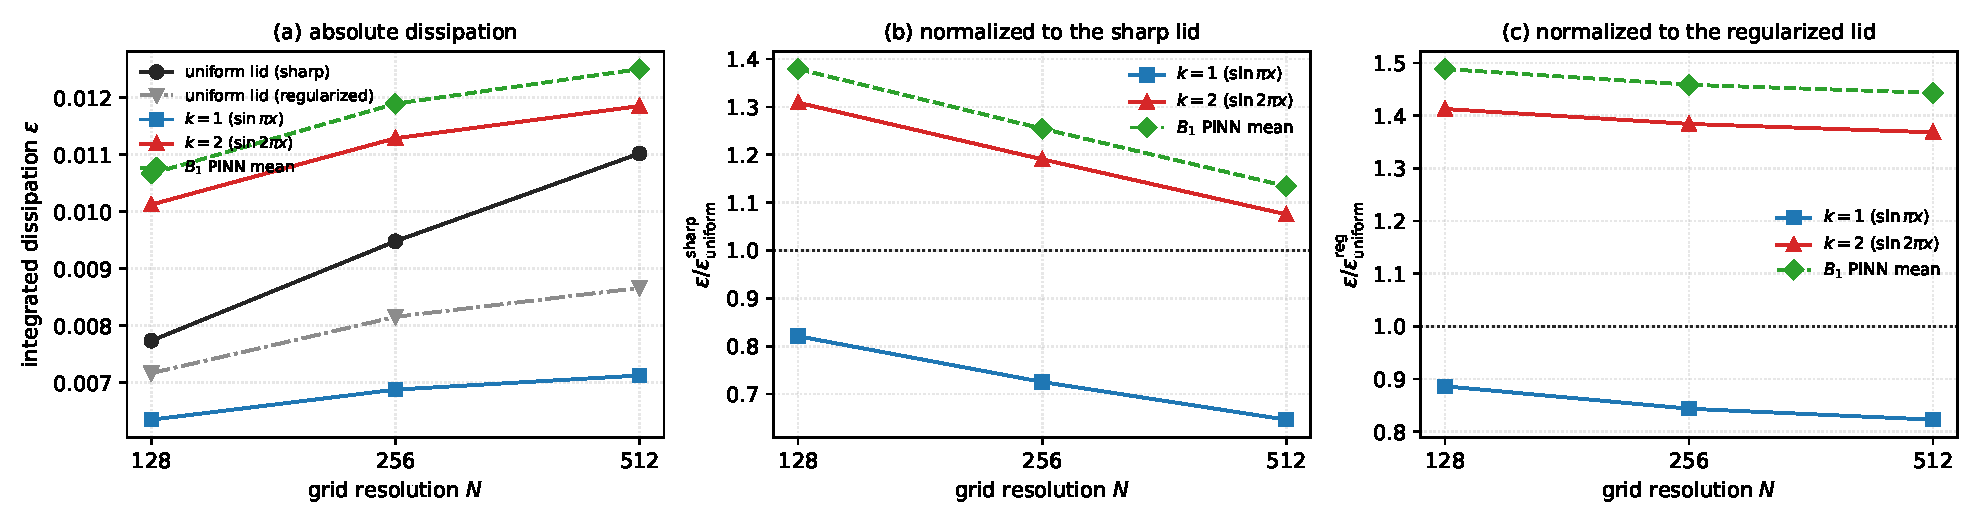
\includegraphics[width=0.92\textwidth]{figures/fig12_gci_updated.pdf}
\caption{Grid convergence of the stationary comparison at $Re=500$ and matched
actuation norm $E^\ast=0.25$. (a) Integrated dissipation versus resolution for the
four stationary controls and for the corner-regularized uniform lid. (b)
Dissipation normalized by the sharp uniform lid on the same grid: this reference
does not converge, and the ratios drift by $18$--$21\%$ over the triple. (c)
Dissipation normalized by the regularized lid: the three ratio triples are
monotone and converge with GCIs of $1.4$--$3.1\%$. The sign of the ordering
$k=1<\text{uniform}<k=2\approx B_1$ is observed at every resolution in both (b)
and (c); its magnitude is reference-dependent.}
\label{fig:gci}
\end{figure}

\subsection{The corner singularity and the reference dependence}
\label{sec:corner}

The non-convergence of the uniform lid is a property of its corners, not of the
uniform profile as such. Its dissipation grows by $16\%$ between $N=256$ and
$N=512$, the signature of a boundary-layer singularity that the grid cannot
resolve. Replacing the discontinuity by the cosine taper of Eq.~\eqref{eq:taper}
removes $21\%$ of the dissipation at $N=512$ and, more importantly, changes the
growth between the two finest grids from $16\%$ to $6\%$, i.e.\ the expected
first-order rate: $p_{\mathrm{obs}}=0.96$, GCI $7.8\%$, extrapolated
$\varepsilon_\infty=9.20\times10^{-3}$. A continuous lid therefore converges, and
the singular one does not. This has two consequences for the interpretation. First,
a comparison of actuation shapes that uses the discontinuous lid as denominator
mixes the shape effect with a resolution artefact; the regularized reference is
the only one that separates them. Second, the corner is an energetic feature in
its own right: the uniform lid concentrates a large part of its dissipation in two
small regions whose contribution grows with resolution, so any ranking that
depends on the corner peak is resolution-dependent by construction.

The practical conclusion is that two numbers must be reported for each profile,
not one. The sharp-lid ratio answers the question ``what does this actuation do
relative to the classical cavity?'' and is the quantity a reader will compare with
the literature. The regularized ratio answers ``what is the effect of the spatial
shape at fixed actuation norm?'' and is the quantity that supports a physical
statement about shape. Both are given in Table~\ref{tab:stationary}, and the text
uses the second for every claim about ordering or magnitude.

\subsection{Local mechanism of the second-harmonic penalty}
\label{sec:mechanism}

The ranking has a local origin that can be read directly from the fields
(Fig.~\ref{fig:mechanism}). The uniform lid concentrates its dissipation in the
two upper corners, where the imposed tangential velocity jumps to zero: the peak
strain-rate magnitude there is $169$ in units of $U_0/L$, against $15.0$ for
$k=1$ and $23.4$ for $k=2$, and those corner layers are the brightest features of
the dissipation field. Both harmonics remove the jump, and their dissipation is
spread over the lid shear layer and the side walls instead. But the second
harmonic pays for this in the interior. Its lid generates a pair of
counter-rotating cells of nearly equal strength, separated by a wall-to-wall
separatrix at $x=0.5$, each enclosing its own low-strain core; the uniform and
first-harmonic lids recover the classical single primary vortex with a corner
eddy. The reorganization shifts the strain-rate distribution towards larger
values: the interior mean $\langle|\Sij|\rangle$ is $1.450$ for $k=2$, against
$1.039$ for the uniform lid and $1.088$ for $k=1$, a $40\%$ increase at identical
actuation norm.

The trade-off is explicit. The first harmonic removes almost all of the corner
peak ($169$ to $15.0$) at a cost of $4.7\%$ in interior mean strain, and is a net
reduction. The second harmonic removes slightly less of it ($23.4$) while raising
the interior mean by $39.6\%$, and is a net penalty: it buys a symmetric two-cell
state with a stronger interior strain field, and the corner singularity it removes
is not costly enough to compensate. Relative to the uniform lid, the increase in
interior mean strain is only $4.7\%$ for $k=1$, but reaches $39.6\%$ for $k=2$.
The latter increase is approximately 8.4 times larger, even though the second
harmonic does not reduce the peak strain below that of the first harmonic ($23.4$
against $15.0$). Additional identification-sensitivity and control-representation
studies, including loss-term ablation, network-capacity sensitivity,
control-space truncation, aspect-ratio dependence and Fourier versus
modified-Chebyshev parametrizations, are documented in
Supplementary Secs.~S3--S7, Tables~S3--S11 and Figs.~S1--S4.
These studies characterize the robustness of branch identification;
the dissipation ordering discussed here is established independently
by the MRT-LBM calculations and their grid and estimator checks
in Supplementary Secs.~S8.4--S8.7.

\begin{figure}[t]
\centering
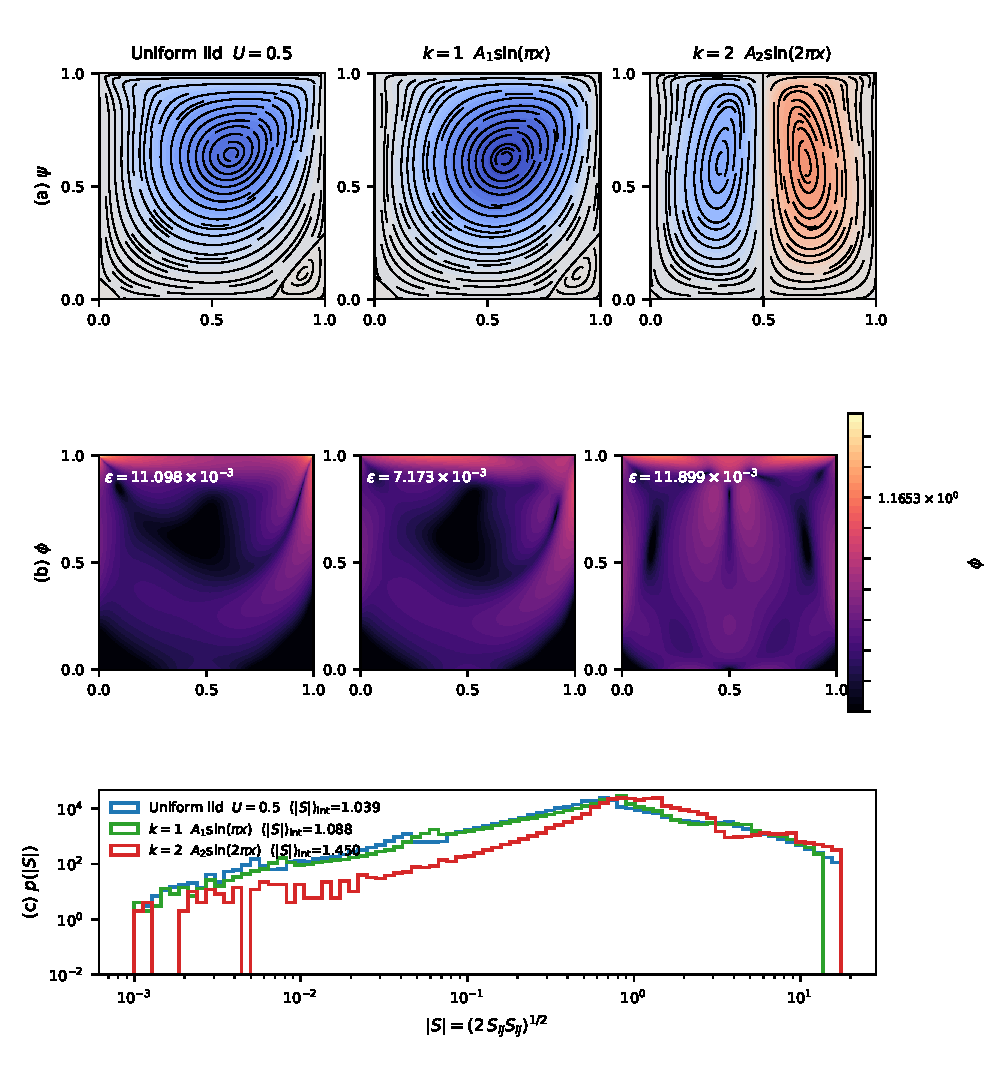
\includegraphics[width=0.78\textwidth]{figures/fig15_mechanism_iso.pdf}
\caption{Local origin of the stationary ranking at $Re=500$, $N=512$ and matched
actuation norm, on scales common to the three columns. (a) Stream function of the
steady response with the streamline topology. (b) Local viscous dissipation
$\phi=\nu(2S_{11}^2+2S_{22}^2+4S_{12}^2)$ on a logarithmic scale spanning six
decades below the global maximum; the annotation gives the domain integral. (c)
Probability density of the strain-rate magnitude over the cavity interior (three
boundary cells excluded), with the interior mean
$\langle|\Sij|\rangle_{\mathrm{int}}$. The uniform lid peaks at the corners
($|\Sij|_{\max}=169$); $k=1$ removes the peak at almost no interior cost
($\langle|\Sij|\rangle_{\mathrm{int}}=1.088$ against $1.039$); $k=2$ removes less
of it ($23.4$) and raises the interior mean to $1.450$, which is the origin of
its dissipation penalty.}
\label{fig:mechanism}
\end{figure}

%----------------------------------------------------------------------
\section{Cycle-mean dissipation of time-dependent actuation branches}
\label{sec:branches_results}
%----------------------------------------------------------------------

\subsection{Why the dissipation of the mean flow is not the cycle mean}

For the stationary controls of Sec.~\ref{sec:stationary} the distinction between
$D(\overline{\mathbf{u}})$ and $\Dbar$ is empty, because the response is steady.
For the time-dependent branches it becomes the central issue. Equation
\eqref{eq:jensen} is exact: the cycle mean exceeds the mean-field value by the
dissipation of the fluctuations, and there is no reason for that term to be small
when the actuation reverses sign. A mean-field diagnostic answers the question
``how much would this flow dissipate if it were steady?''; it does not answer
``how much does it dissipate?''. Figure~\ref{fig:cycle} and
Table~\ref{tab:cycle} show how far apart the two answers can be; supplementary
Tables~S15--S16 provide additional cycle-averaged statistics and iso-energetic
comparisons, while Figs.~S5--S6 provide the phase-resolved field captures.

\begin{figure}[t]
\centering
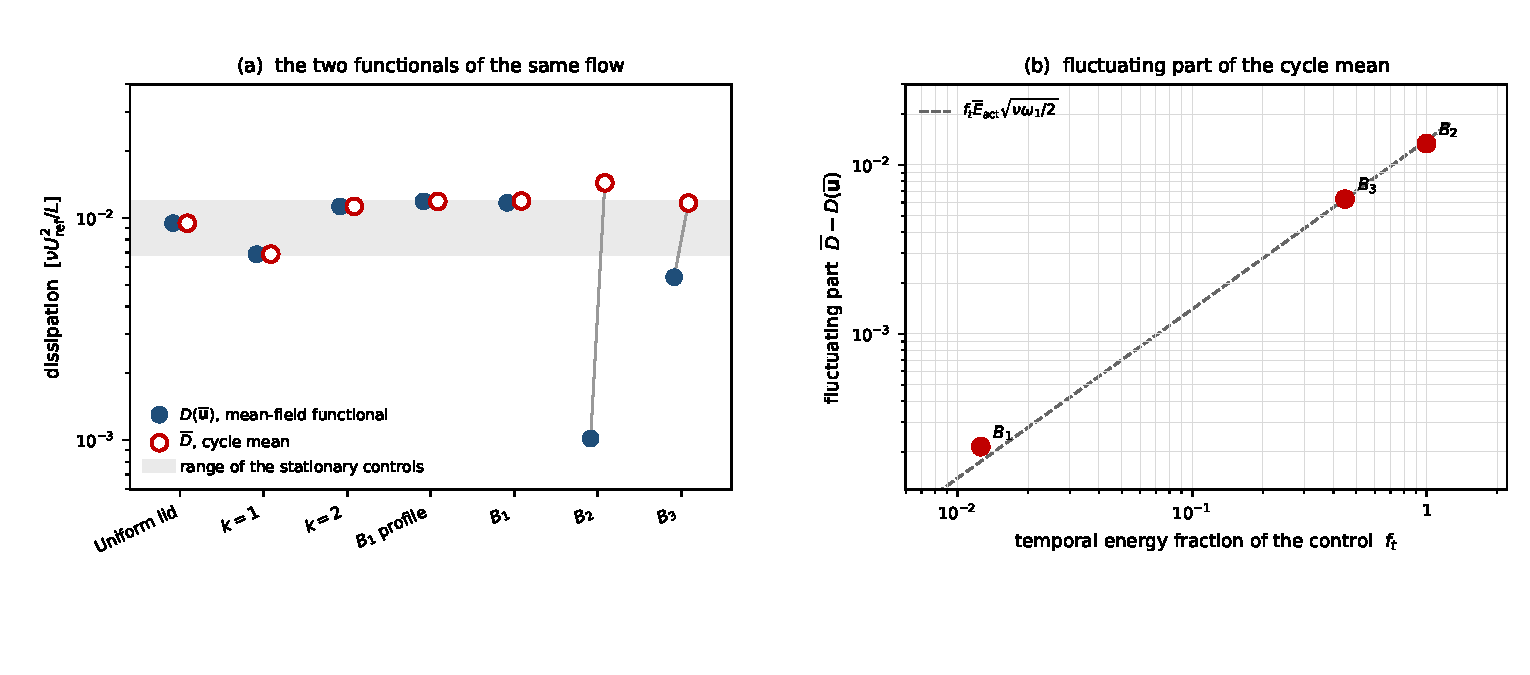
\includegraphics[width=0.94\textwidth]{figures/fig18_branch_iso_cycle.pdf}
\caption{Iso-energetic comparison of the nine controls at $Re=500$,
$\overline{E}_{\mathrm{act}}=0.25$ and $N=256$. Left: the two dissipation
functionals of each control, the dissipation of the time-mean field (filled
markers) and the cycle mean (open markers), joined by the gap between them; the
two coincide for stationary controls. Right: cycle-mean dissipation against the
temporal energy fraction $f_t$ of the lid control. The ordering in $f_t$ is the
order in which the branches are recovered by the identification, and it is not the
order of the dissipation cost.}
\label{fig:cycle}
\end{figure}

\subsection{Cycle-mean comparison of the three branches}
\label{sec:branch_compare}

Table~\ref{tab:cycle} collects the result. The five quasi-stationary controls span
less than a factor of two, from $6.88\times10^{-3}$ for $k=1$ to
$1.22\times10^{-2}$ for the full $B_1$ series, and their mean-field and cycle-mean
values coincide to within $4\%$; for the $B_1$ series the difference is
$1.17\times10^{-2}$ against $1.22\times10^{-2}$, which is the residual effect of
its small temporal content. The branches with substantial temporal content leave
that band. $B_2$ dissipates $3.76\times10^{-2}$ over the cycle while its mean
field dissipates $3.10\times10^{-5}$, a ratio of $1214$; its mean field holds only
$6\%$ of the cycle-mean kinetic energy, so the mean motion is a shallow
recirculation under the lid, not a weakened copy of the instantaneous flow. $B_3$
is intermediate: $D(\overline{\mathbf{u}})=5.05\times10^{-3}$ and
$\Dbar=2.18\times10^{-2}$, a ratio of $4.3$. On the cycle average, and at the same
actuation norm, $B_2$ costs $3.1$ times $B_1$ and $5.5$ times the least
dissipative stationary control; its two realizations agree to $1.7\%$, whereas the
two $B_3$ realizations differ by $23\%$, so the $B_3$ value quoted here is the
lower of the two and must be read as a lower bound on that class.

\begin{table}[t]
\centering
\caption{Dissipation of the time-mean field and cycle-mean dissipation at
$Re=500$, $N=256$ and cycle-mean actuation norm $\overline{E}_{\mathrm{act}}=0.25$.
$D(\overline{\mathbf{u}})$ is the functional evaluated on the time-mean field;
$\Dbar$ is the average of the instantaneous dissipation over the phase-resolved
periodic response and is the performance index relevant to a periodic flow. The
two coincide only in the steady limit. $A_\varepsilon$ is the half-spread of
$D(t)$ over the cycle, i.e.\ the variability concealed by a single cycle-mean
number. The $B_1$ mean profile row is stationary by construction; the $B_1$ full
row is the identified series.}
\label{tab:cycle}
\small
\begin{tabular}{lcccccc}
\toprule
Control & $f_t$ & $\overline{E}_{\mathrm{act}}$ & $D(\overline{\mathbf{u}})$ & $\Dbar$
& $\Dbar/D(\overline{\mathbf{u}})$ & $A_\varepsilon$\\
\midrule
Uniform lid & 0.000 & 0.250 & $9.48\times10^{-3}$ & $9.48\times10^{-3}$ & 1.00 & $0$\\
$k=1$ ($\sin\pi x$) & 0.000 & 0.250 & $6.88\times10^{-3}$ & $6.88\times10^{-3}$ & 1.00 & $0$\\
$k=2$ ($\sin 2\pi x$) & 0.000 & 0.250 & $1.13\times10^{-2}$ & $1.13\times10^{-2}$ & 1.00 & $0$\\
$B_1$ mean profile & 0.000 & 0.250 & $1.19\times10^{-2}$ & $1.19\times10^{-2}$ & 1.00 & $0$\\
$B_1$ full series & 0.074 & 0.250 & $1.17\times10^{-2}$ & $1.22\times10^{-2}$ & 1.04 & $2.4\times10^{-3}$\\
$B_2$ seed 5 & 0.998 & 0.250 & $3.10\times10^{-5}$ & $3.76\times10^{-2}$ & 1214 & $3.6\times10^{-2}$\\
$B_2$ seed 14 & 0.975 & 0.250 & $1.82\times10^{-4}$ & $3.70\times10^{-2}$ & 204 & $3.5\times10^{-2}$\\
$B_3$ seed 0 & 0.448 & 0.250 & $5.05\times10^{-3}$ & $2.18\times10^{-2}$ & 4.3 & $1.5\times10^{-2}$\\
$B_3$ seed 4 & 0.637 & 0.250 & $3.12\times10^{-3}$ & $2.69\times10^{-2}$ & 8.6 & $2.6\times10^{-2}$\\
\bottomrule
\end{tabular}
\end{table}

Three statements follow, and they are the ones the paper retains. First, the
mean-field functional is not a surrogate for the cycle mean: it can be three
orders of magnitude too small and it reverses the ranking of the branches. Second,
the temporal fraction $f_t$ orders the branches by accessibility, not by cost:
$B_2$, the most strongly time-dependent control, is the most dissipative of the
three at matched norm. Third, the ranking of the time-dependent branches
($B_1<B_3<B_2$) is the same as the ranking of their mean-field dissipation read in
reverse, which is a direct consequence of Eq.~\eqref{eq:jensen}: the branch that
suppresses its mean flow most effectively is the one that pays most in
fluctuations.

\subsection{Flow organization behind the cycle-mean cost}
\label{sec:topology}

The field-level organization explains the numbers (Figs.~\ref{fig:topology}
and~\ref{fig:velocity}). The $B_1$ time-mean flow is the familiar pair of
counter-rotating cells centred at $(0.31,0.54)$ and $(0.69,0.56)$, with
$\max|\langle\mathbf{u}\rangle|=0.733$ and $\langle\psi\rangle\in[-0.036,0.035]$;
half of its mean kinetic energy lies below $y=0.675$, so the cells fill the
cavity. Its instantaneous states coincide with that mean to $2.7\%$ in field norm
and its kinetic-energy fluctuation ratio is $R_K=4\times10^{-4}$, so it is
quasi-stationary in the operational sense. The $B_2$ mean field is $19$ times
weaker in stream function ($\max|\langle\psi\rangle|=0.0019$) and $18$ times weaker
in peak speed ($0.042$, or $5.7\%$ of the $B_1$ value); its mean extrema sit at
$y=0.89$--$0.92$ and half of the mean kinetic energy lies above $y=0.95$. Its
streamwise fluctuation, by contrast, reaches $0.555$---thirteen times its own mean
and $76\%$ of the $B_1$ mean peak. The $B_3$ flow keeps an intermediate mean
circulation ($\max|\langle\mathbf{u}\rangle|=0.595$, $81\%$ of $B_1$) but places
it close to the lid, with extrema at $(0.20,0.86)$ and $(0.77,0.81)$ and half of
the mean kinetic energy above $y=0.91$; its fluctuation reaches $0.416$.

``Weak mean flow'' is therefore not ``weak flow''. The controls with a strong
temporal component do not produce a small perturbation around a mean
recirculation: they produce responses whose fluctuations dominate the
instantaneous field while the mean is nearly zero. A figure that normalized each
panel by its own maximum, or a diagnostic that used only the mean field, would
hide exactly the contrast that defines the two unsteady branches.

\begin{figure}[t]
\centering
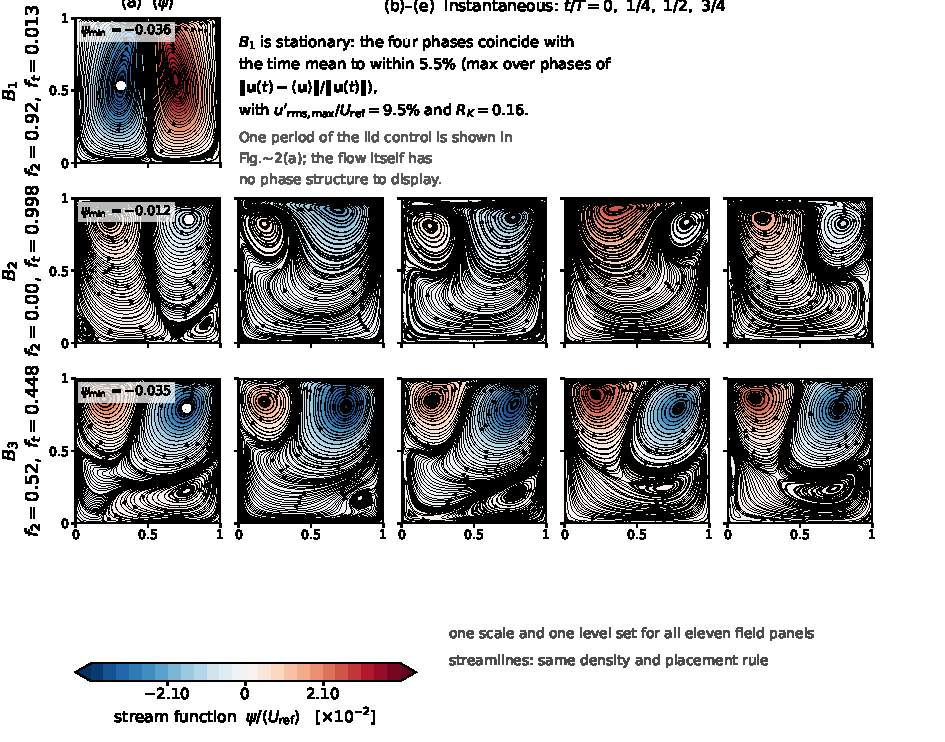
\includegraphics[width=\textwidth]{figures/fig20_branch_topology.pdf}
\caption{Flow topology of the three branch controls at $Re=500$,
$E^\ast=0.25$ and $N=256$, on one stream-function scale and one set of contour
levels common to all panels. Rows: $B_1$ (full series, $f_t=0.074$), $B_2$
(seed 5, $f_t=0.998$) and $B_3$ (seed 0, $f_2=0.520$, $f_t=0.448$). (a) Time mean
$\langle\psi\rangle$ with the streamlines of the mean flow; the circle marks its
negative extremum. (b)--(e) Instantaneous $\psi$ and streamlines at
$t/T=0,1/4,1/2,3/4$ for $B_2$ and $B_3$; the four phases belong to the same
periodic state, whose first- and second-half phase averages differ by at most
$1.0\times10^{-3}$ in relative field norm. For $B_1$ the instantaneous states
coincide with the mean to $2.7\%$, so the four panels are replaced by that
statement. The common scale is deliberate: the $B_2$ mean cell is $19$ times
weaker than the $B_1$ one and is nearly invisible, which is the point.}
\label{fig:topology}
\end{figure}

\begin{figure}[t]
\centering
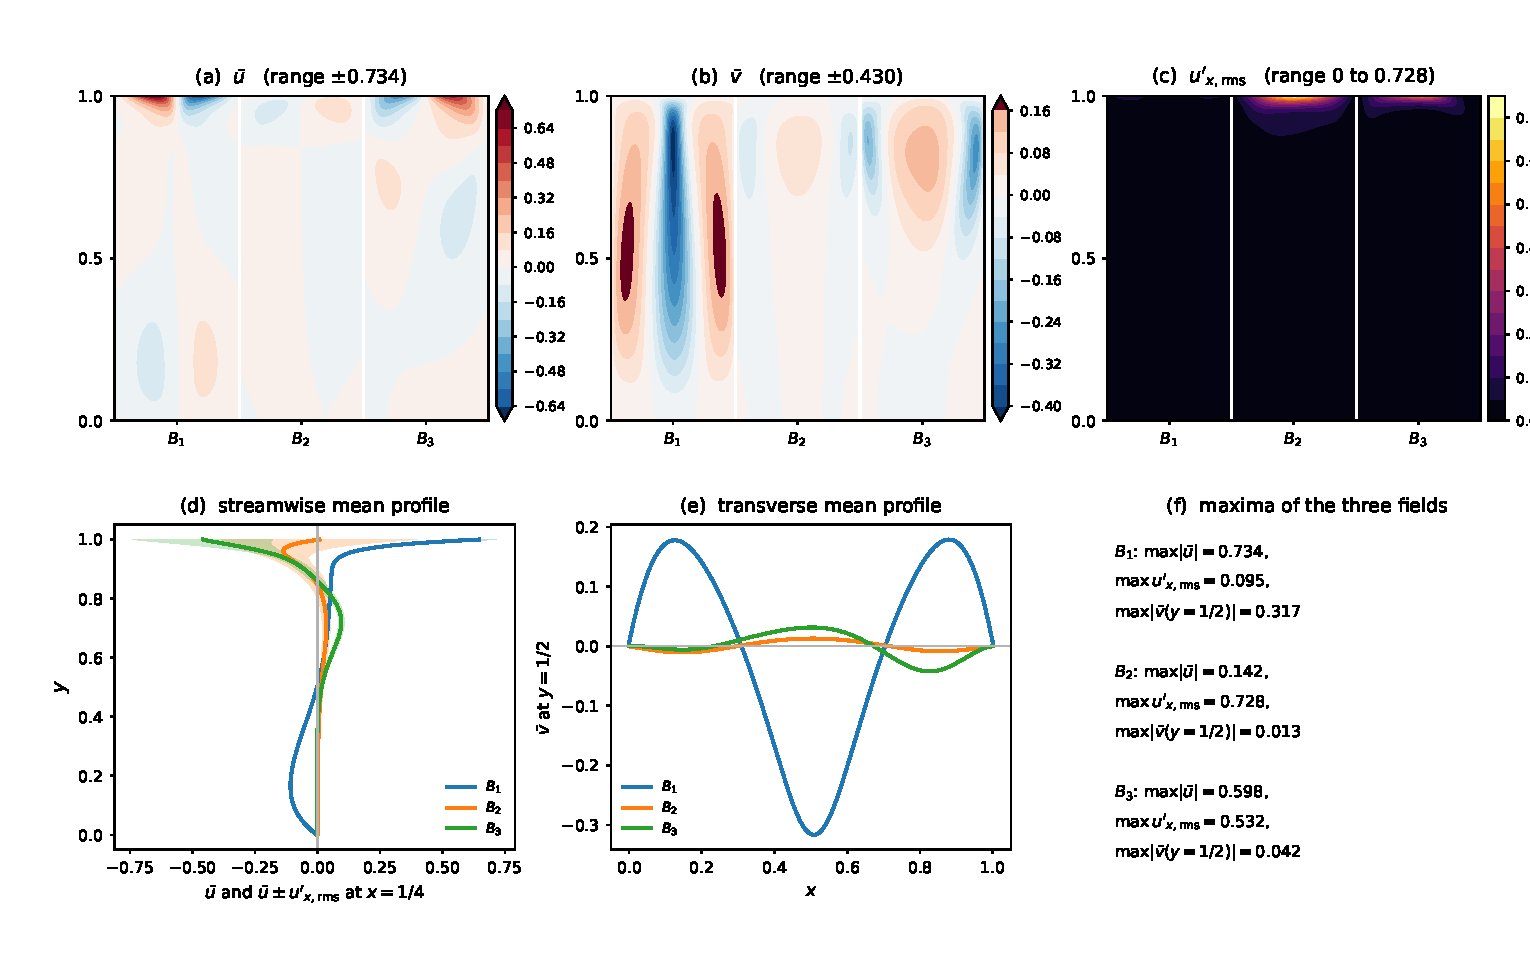
\includegraphics[width=0.92\textwidth]{figures/fig21_branch_velocity.pdf}
\caption{Velocity fields and centreline profiles of the same three captures.
Rows: (a) $\bar u$, (b) $\bar v$ and (c) $u'_{x,\mathrm{rms}}$, each on one colour
range for the three columns and a single normalization, with the occupied range
written in every panel so that the common scale can be checked. Grey lines are the
zero contours of the mean fields. (d) $\bar u$ along $x=1/4$ with the
$\pm u'_{\mathrm{rms}}$ band; the midline $x=1/2$ is not used because the
antisymmetric controls have $u\equiv0$ there. (e) $\bar v$ along $y=1/2$, with
$\bar v$ on the abscissa. The bands are temporal standard deviations over the
sixty-four sampled periods, not confidence intervals.}
\label{fig:velocity}
\end{figure}

\subsection{Mechanical energy budget of the branches}
\label{sec:budget}

Table~\ref{tab:budget} and Fig.~\ref{fig:energy} close the comparison with the
budget of Eq.~\eqref{eq:budget}. The kinetic energy separates the branches by two
orders of magnitude ($1.15\times10^{-2}$, $2.47\times10^{-4}$ and
$3.98\times10^{-3}$), while the cycle-mean dissipation orders them the other way
round ($1.22\times10^{-2}$, $3.76\times10^{-2}$ and $2.18\times10^{-2}$). Within
the period, $D(t)$ varies by a factor $1.5$, $10.9$ and $4.2$ respectively, and
the lid power of $B_2$ is negative for $14\%$ of the period: the flow returns
energy through the lid while the Stokes layer spins down. The residual
$\overline{P}_{\mathrm{lid}}-\Dbar$, computed with the wall velocity recovered at
the boundary node rather than the prescribed profile (Sec.~S8.7), is
$-2.9\%$, $-0.1\%$ and $-0.9\%$.

\begin{table}[t]
\centering
\caption{Mechanical energy budget of the three branch controls at $Re=500$ and
$N=256$, at the common cycle-mean actuation norm $E^\ast=0.25$: $B_1$ is the full
series ($f_t=0.074$), $B_2$ is seed 5 ($f_t=0.998$) and $B_3$ is seed 0
($f_2=0.520$, $f_t=0.448$). All quantities are cycle averages over 64 forced
periods of the instantaneous fields; $\Dbar$ is never replaced by
$D(\overline{\mathbf{u}})$. $\sigma(\Dbar)$ is the block standard error over eight
blocks of eight cycles, expanded by $t_{7,0.975}=2.365$; it is below $0.1\%$ for
all three branches because the response is periodic to better than $10^{-3}$, so
the physically relevant uncertainty is the seed-to-seed spread ($1.7\%$ within
$B_2$, $23\%$ within $B_3$). The residual
$\overline{P}_{\mathrm{lid}}-\Dbar$ is the first-order truncation of the wall-shear
estimator, not a physical imbalance (Sec.~\ref{sec:budget}).}
\label{tab:budget}
\small
\begin{tabular}{lccccc}
\toprule
Branch & $\overline{E}_{\mathrm{act}}$ & $\overline{K}$ & $\overline{P}_{\mathrm{lid}}$
& $\Dbar$ & $\sigma(\Dbar)$\\
\midrule
$B_1$ (full series) & 0.2500 & $1.15\times10^{-2}$ & $1.18\times10^{-2}$ & $1.22\times10^{-2}$ & $<0.1\%$\\
$B_2$ (seed 5) & 0.2504 & $2.47\times10^{-4}$ & $3.76\times10^{-2}$ & $3.76\times10^{-2}$ & $<0.1\%$\\
$B_3$ (seed 0) & 0.2503 & $3.98\times10^{-3}$ & $2.16\times10^{-2}$ & $2.18\times10^{-2}$ & $<0.1\%$\\
\bottomrule
\end{tabular}
\end{table}

The residual is two to three orders of magnitude larger than the drift of $K$ over
the sampling window, which is at most $1.5\times10^{-2}\%$ of $\Dbar$; it is
therefore not a failure of periodicity. It is the truncation error of the
one-sided wall-shear estimate. Two checks bound that error. First, the first-order
estimator reproduces the independently accumulated $\Plid$ of the same fields to
$0.3\%$ for $B_1$, so it is internally consistent; the residual is a property of
the estimator, not of the accumulation. Second, replacing it by a second-order
one-sided derivative on the same fields moves the $B_1$ mean-field residual from
$-2.87\%$ to $+0.58\%$, i.e.\ it crosses zero, which shows that the estimator
uncertainty is of the order of the residual itself (a few per cent). Applied to
the branch cycle means, the same change moves the $B_1$ residual to $+1.4\%$ but
inflates the $B_2$ and $B_3$ residuals, because the three-point stencil amplifies
lattice-scale noise in the thin Stokes layer. We therefore retain the first-order
estimator for all three branches, report the residual as measured, and present
Eq.~\eqref{eq:closure} as an energetic verification with a few-per-cent estimator
uncertainty rather than as an exact closure. This is sufficient for the
conclusions drawn here, which rest on differences of a factor of three, not on
the third significant digit.

\begin{figure}[t]
\centering
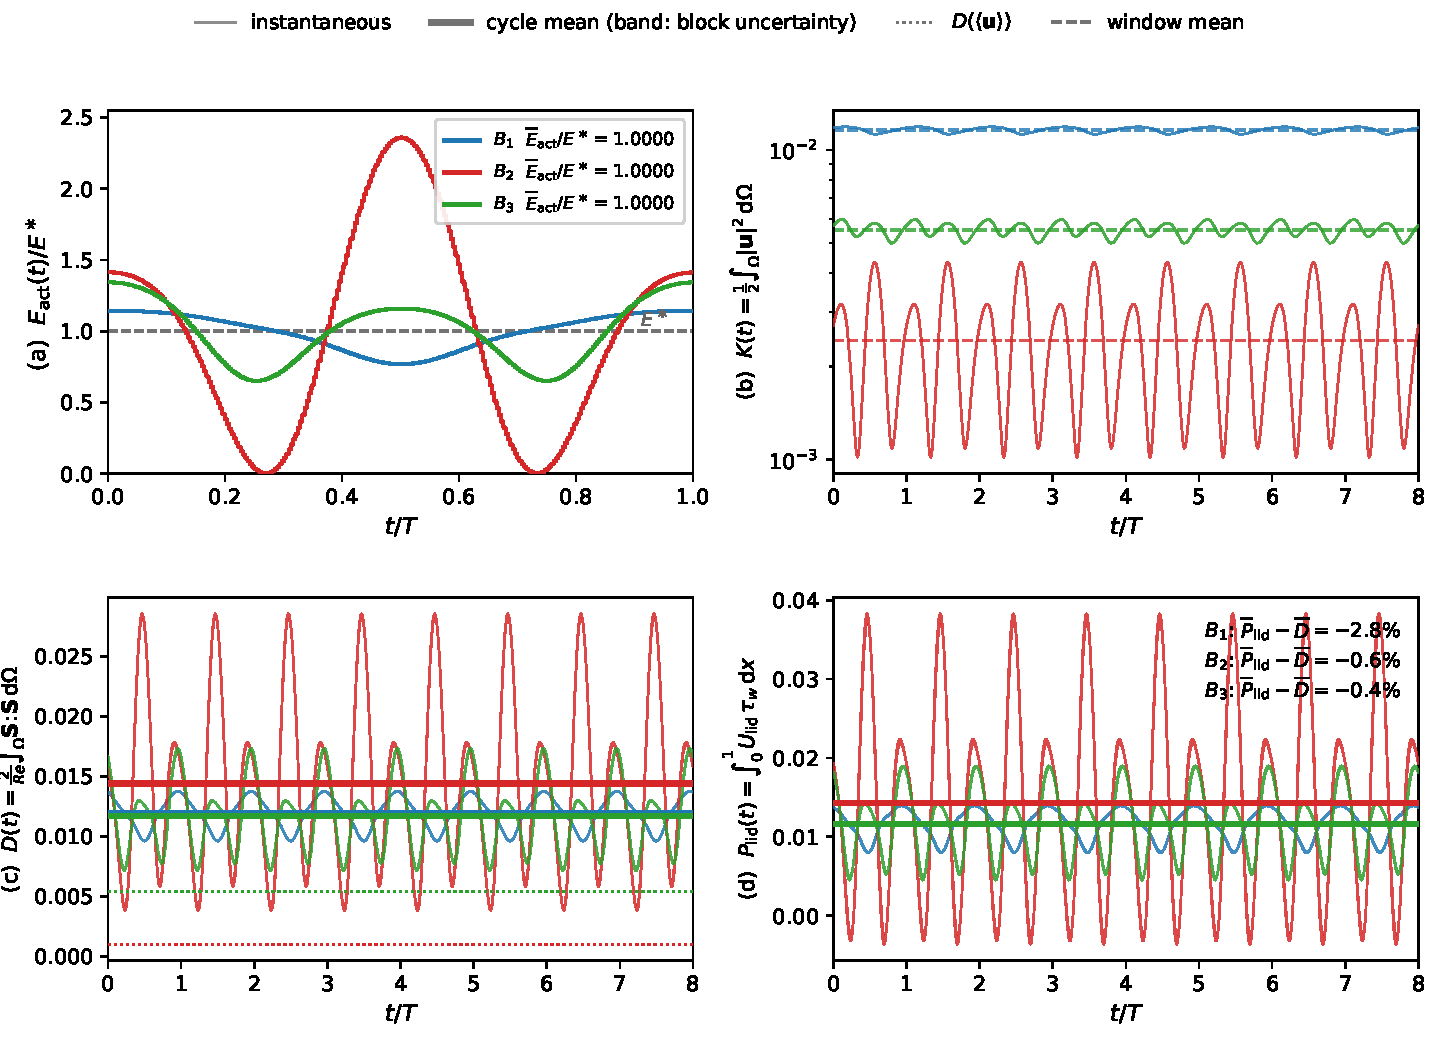
\includegraphics[width=\textwidth]{figures/fig22_branch_energy.pdf}
\caption{Phase-resolved energetic response of the three branches at $Re=500$ and
$E^\ast=0.25$. (a) Instantaneous actuation norm $\Eact(t)$ over one forced period,
normalized by the common cycle-mean target. (b) Kinetic energy $K(t)$ over the
first eight of the sixty-four sampled periods (logarithmic ordinate). (c) Viscous
dissipation $D(t)$: instantaneous (thin), cycle mean (thick, with the block
uncertainty as a band) and, dotted, the dissipation $D(\langle\mathbf{u}\rangle)$
of the time-mean field, which is not substituted for the cycle mean. (d) Lid power
$\Plid(t)$, positive into the fluid, with the same conventions; the annotations
give the window-averaged residual $\overline{P}_{\mathrm{lid}}-\Dbar$ computed
with the recovered wall velocity (Sec.~S8.7). The
kinetic-energy balance integrates to zero over one period of a periodic state, so
the two cycle means must agree; the measured residual is the wall-shear estimator
error discussed in the text.}
\label{fig:energy}
\end{figure}

%----------------------------------------------------------------------
\section{Physical interpretation and implications for flow control}
\label{sec:interpretation}
%----------------------------------------------------------------------

\subsection{Why the stationary second harmonic increases dissipation}

At matched quadratic actuation norm the second harmonic is not a low-dissipation
mode, and the reason is geometric rather than spectral. The lid profile
$A_2\sin(2\pi x)$ imposes two opposite lobes of wall velocity, which drive two
counter-rotating cells of comparable strength instead of one primary vortex. That
reorganization has two competing energetic consequences. It removes the corner
velocity jump, which suppresses a singular strain peak that dominates the
dissipation of the uniform lid. It also forces the return flow through a
wall-to-wall separatrix at the cavity centre, which raises the strain over the
whole interior: the interior mean of $|\Sij|$ increases by $40\%$ at identical
norm. The second effect wins, because the corner layer is thin while the interior
is not. The first harmonic removes the same corner peak at almost no interior
cost, and is the only stationary profile that is a net reduction. The energetic
cost of a spatial actuation mode is thus controlled by the volume over which it
raises the strain, not by the peak it removes; a mode that is ``smoother'' at the
wall need not be less dissipative in the bulk.

\subsection{Why temporal forcing increases the cycle-mean dissipation}

For a periodic control the relevant functional is the cycle mean of a quadratic
quantity, and the fluctuations are a first-order contribution to it, not a
correction. Equation~\eqref{eq:jensen} makes this explicit, and the $B_2$ branch
is its clearest illustration: a mean field that dissipates $3.1\times10^{-5}$ and
a cycle mean that dissipates $3.8\times10^{-2}$, with the mean field holding $6\%$
of the kinetic energy. The physical reason is that the oscillating lid generates a
Stokes layer whose wall-normal gradients are large and reverse twice per period;
the instantaneous strain is therefore large wherever the instantaneous velocity
is large, and the time average of its square cannot be recovered from the average
velocity. The same mechanism explains why the lid power of $B_2$ is negative for
$14\%$ of the period: while the Stokes layer spins down, the flow pushes the wall
and returns part of the energy that it received earlier. A control designer who
evaluates such a state from its mean field will conclude that it is almost
frictionless, whereas the cycle average ranks it as the most dissipative of the
three branches.

\subsection{What branch accessibility does and does not imply}

The three branches were not selected by their dissipation. They were selected by a
physics-informed optimization whose loss contains a dissipation objective, an
actuation-norm constraint and a spatial-variance regularizer, and whose outcome
depends on the initialization and on the regularization weight
\cite{beniaiche2026}. At $Re=500$ and $E^\ast=0.25$ the stationary
second-harmonic structure is the most frequently recovered one, and the full
$B_1$ series is quasi-stationary and reproducible; that is a statement about the
variational landscape, and it is confirmed here by the independent solver. It is
not a statement about efficiency. At the same actuation norm the branch most
frequently recovered is a net dissipation penalty relative to the first harmonic,
and the branch with the strongest temporal content, which is also recovered in a
reproducible way, is the most dissipative of the three. The operational
conclusion is that accessibility and physical performance are different
properties, and that a control study which reports only the recovered mode, or
only its mean-field dissipation, can invert the energetic ranking of the
actuations it compares.

Two limits of this statement must be stated explicitly, because they define its
scope. First, the temporal comparison covers three representative realizations at
a single Reynolds number ($Re=500$) and a single grid ($N=256$), with two
realizations for $B_2$ and $B_3$; the within-class spread is $1.7\%$ for $B_2$ but
$23\%$ for $B_3$, so the $B_3$ cost is a lower bound on its class. The stationary
comparison, by contrast, rests on three grids and two reference lids. Second, the
$B_1$ temporal content is small but not zero ($f_t=0.074$), and its cycle mean
exceeds its mean-field value by $4\%$; the quasi-stationary limit is approached,
not attained. Generalization to other Reynolds numbers, to three-dimensional
cavities, or to actuations with a different spatial support is not implied by the
present results.

%----------------------------------------------------------------------
\section{Conclusions}
\label{sec:conclusions}
%----------------------------------------------------------------------

Four statements summarize the study.

\begin{enumerate}
\item \emph{The spatial structure of wall actuation reorganizes the cavity and the
strain field.} At matched quadratic actuation norm the second spatial harmonic
replaces the single primary vortex of the uniform lid by two counter-rotating
cells and raises the interior mean strain rate by $40\%$; the first harmonic
removes the corner strain peak at almost no interior cost. The corner singularity
of the discontinuous lid is an energetic feature in its own right: it prevents the
convergence of the reference dissipation ($p_{\mathrm{obs}}=0.18$,
GCI $131\%$) and disappears once the corner is regularized
($p_{\mathrm{obs}}=0.96$, GCI $7.8\%$).
\item \emph{The ranking of stationary profiles depends on the constraint.} At
equal actuation norm, and relative to a converged corner-regularized reference,
the first harmonic reduces the dissipation by $17.7\%$, while the second harmonic
and the mean profile of the identified stationary branch increase it by $36.8\%$
and $44.3\%$. At equal lid speed the same three profiles are all less dissipative
than the uniform lid and the second harmonic is the best of them
\cite{beniaiche2026}; the inversion is produced by the norm constraint, which
fixes the rms wall velocity but not the peak, and therefore not the effective
Reynolds number ($Re_{\max}=250$ for the uniform lid, $354$ for the harmonics,
$390$ for the $B_1$ mean profile at $E^\ast=0.25$).
\item \emph{The cycle-mean dissipation of a time-dependent actuation is not the
dissipation of its mean field.} For the temporally dominated branch the two
differ by a factor $1214$, and the branch that is most strongly damped in the mean
is the most dissipative on the cycle ($3.76\times10^{-2}$, i.e.\ $3.1$ times the
quasi-stationary branch and $5.5$ times the first harmonic). The fluctuating part
of the strain field carries the cost, and Eq.~\eqref{eq:jensen} makes that
statement exact.
\item \emph{The branch recovered by optimization is not the branch that minimizes
dissipation at fixed control effort.} The most frequently recovered stationary
structure is a net penalty at matched norm, and the most strongly time-dependent
branch is the most dissipative of the three. Accessibility, reproducibility and
physical performance are distinct properties of an actuation, and only the last is
measured by the cycle-mean dissipation.
\end{enumerate}

The practical implication for modal flow control is that a comparison of actuation
strategies must state its constraint explicitly. Equal wall speed, equal quadratic
norm and equal mechanical power define three different problems and can produce
three different rankings; the present study uses the quadratic norm because it is
the constraint available to an optimizer, and reports the peak velocity so that
the effective Reynolds number of each comparison is visible. The cycle-mean
dissipation, not the mean-field value and not the modal spectrum, is the
performance index that follows from the energy identity.

Three extensions follow directly. A grid study of the time-dependent branches
would establish whether the factor-of-three separation is resolution-independent
to the same degree as the stationary ranking. Retraining under an explicit
cycle-mean norm constraint, rather than rescaling an identified control after the
fact, would separate the effect of the constraint from the effect of the
identification path. Finally, three-dimensional cavities would introduce spanwise
modes and test whether the two-cell second-harmonic state survives when the flow
can vary along the span. The physics-informed identification remains, in this
programme, the tool that generates the candidate actuations; the fluid-mechanical
evaluation is what decides between them.

%----------------------------------------------------------------------
\section*{Data availability}
%----------------------------------------------------------------------

The actuation series, the field captures and the post-processing scripts that
support the figures and tables of this article are available at
\url{https://github.com/Ahmedalgeria778/PoF_cavity_dissipation_study} and from the
corresponding author on reasonable request.

\section*{Acknowledgments}
The authors thank the Laboratory of Fluid Mechanics of the Ecole Militaire
Polytechnique for computational support.

\begin{thebibliography}{99}

\bibitem{ghia1982high}
U.~Ghia, K.~N.~Ghia, and C.~T.~Shin,
``High-Re solutions for incompressible flow using the Navier--Stokes equations and
a multigrid method,'' J.\ Comput.\ Phys.\ \textbf{48}, 387--411 (1982).

\bibitem{botella1998benchmark}
O.~Botella and R.~Peyret,
``Benchmark spectral results on the lid-driven cavity flow,''
Comput.\ Fluids \textbf{27}, 421--433 (1998).

\bibitem{shankardeshpande2000}
P.~N.~Shankar and M.~D.~Deshpande,
``Fluid mechanics in the driven cavity,''
Annu.\ Rev.\ Fluid Mech.\ \textbf{32}, 93--136 (2000).

\bibitem{albensoeder2005accurate}
S.~Albensoeder and H.~C.~Kuhlmann,
``Accurate three-dimensional lid-driven cavity flow,''
J.\ Comput.\ Phys.\ \textbf{206}, 536--558 (2005).

\bibitem{kuhlmann2019}
H.~C.~Kuhlmann and F.~Roman\`o,
``The lid-driven cavity,'' in \textit{Computational Modelling of Bifurcations and
Instabilities in Fluid Dynamics}, edited by A.~Gelfgat (Springer, Cham, 2019),
pp.~233--309.

\bibitem{gadelhak2000}
M.~Gad-el-Hak,
\textit{Flow Control: Passive, Active, and Reactive Flow Management}
(Cambridge University Press, Cambridge, 2000).

\bibitem{brunton2015closed}
S.~L.~Brunton and B.~R.~Noack,
``Closed-loop turbulence control: Progress and challenges,''
Appl.\ Mech.\ Rev.\ \textbf{67}, 050801 (2015).

\bibitem{rowley2017model}
C.~W.~Rowley and S.~T.~M.~Dawson,
``Model reduction for flow analysis and control,''
Annu.\ Rev.\ Fluid Mech.\ \textbf{49}, 387--417 (2017).

\bibitem{bewley2001dns}
T.~R.~Bewley, P.~Moin, and R.~Temam,
``DNS-based predictive control of turbulence: an optimal benchmark for feedback
algorithms,'' J.\ Fluid Mech.\ \textbf{447}, 179--225 (2001).

\bibitem{bergmann2005optimal}
M.~Bergmann, L.~Cordier, and J.-P.~Brancher,
``Optimal rotary control of the cylinder wake using proper orthogonal
decomposition reduced-order model,'' Phys.\ Fluids \textbf{17}, 097101 (2005).

\bibitem{choi1994active}
H.~Choi, P.~Moin, and J.~Kim,
``Active turbulence control for drag reduction in wall-bounded flows,''
J.\ Fluid Mech.\ \textbf{262}, 75--110 (1994).

\bibitem{quadrio2004critical}
M.~Quadrio and P.~Ricco,
``Critical assessment of turbulent drag reduction through spanwise wall
oscillations,'' J.\ Fluid Mech.\ \textbf{521}, 251--262 (2004).

\bibitem{corke2010dbd}
T.~C.~Corke, C.~L.~Enloe, and S.~P.~Wilkinson,
``Dielectric barrier discharge plasma actuators for flow control,''
Annu.\ Rev.\ Fluid Mech.\ \textbf{42}, 505--529 (2010).

\bibitem{rabsult2019drl}
J.~Rabault, M.~Kuchta, A.~Jensen, U.~R\'eglade, and N.~Cerardi,
``Artificial neural networks trained through deep reinforcement learning discover
control strategies for active flow control,''
J.\ Fluid Mech.\ \textbf{865}, 281--302 (2019).

\bibitem{garnier2021drl}
P.~Garnier, J.~Viquerat, J.~Rabault, A.~Larcher, A.~Kuhn, and E.~Hachem,
``A review on deep reinforcement learning for fluid mechanics,''
Comput.\ Fluids \textbf{225}, 104973 (2021).

\bibitem{raissi2019pinn}
M.~Raissi, P.~Perdikaris, and G.~E.~Karniadakis,
``Physics-informed neural networks: A deep learning framework for solving forward
and inverse problems involving nonlinear partial differential equations,''
J.\ Comput.\ Phys.\ \textbf{378}, 686--707 (2019).

\bibitem{cai2021pinnreview}
S.~Cai, Z.~Mao, Z.~Wang, M.~Yin, and G.~E.~Karniadakis,
``Physics-informed neural networks (PINNs) for fluid mechanics: A review,''
Acta Mech.\ Sin.\ \textbf{37}, 1727--1738 (2021).

\bibitem{noack2003hierarchy}
B.~R.~Noack, K.~Afanasiev, M.~Morzy\'nski, G.~Tadmor, and F.~Thiele,
``A hierarchy of low-dimensional models for the transient and post-transient
cylinder wake,'' J.\ Fluid Mech.\ \textbf{497}, 335--363 (2003).

\bibitem{schmid2010dmd}
P.~J.~Schmid,
``Dynamic mode decomposition of numerical and experimental data,''
J.\ Fluid Mech.\ \textbf{656}, 5--28 (2010).

\bibitem{taira2017modal}
K.~Taira, C.~W.~Rowley, O.~T.~Schmidt, D.~S.~Luchtenburg, S.~L.~Brunton, and
B.~R.~Noack,
``Modal analysis of fluid flows: An overview,''
AIAA J.\ \textbf{55}, 4013--4041 (2017).

\bibitem{sipp2010global}
D.~Sipp and A.~Lebedev,
``Global stability of base and mean flows: a general approach and its applications
to cylinder and open cavity flows,'' J.\ Fluid Mech.\ \textbf{593}, 333--358 (2007).

\bibitem{beneddine2016conditions}
S.~Beneddine, D.~Sipp, A.~Arnault, J.~Dandois, and F.~Lesshafft,
``Conditions for validity of mean flow stability analysis,''
J.\ Fluid Mech.\ \textbf{798}, 485--504 (2016).

\bibitem{pope2000}
S.~B.~Pope, \textit{Turbulent Flows} (Cambridge University Press, Cambridge, 2000).

\bibitem{landau1987}
L.~D.~Landau and E.~M.~Lifshitz,
\textit{Fluid Mechanics}, 2nd ed. (Pergamon, Oxford, 1987).

\bibitem{doering2002energy}
C.~R.~Doering and C.~Foias,
``Energy dissipation in body-forced turbulence,''
J.\ Fluid Mech.\ \textbf{467}, 289--306 (2002).

\bibitem{dhumieres2002mrt}
D.~d'Humi\`eres,
``Multiple-relaxation-time lattice Boltzmann models in three dimensions,''
Philos.\ Trans.\ R.\ Soc.\ Lond.\ A \textbf{360}, 437--451 (2002).

\bibitem{chen1998doolen}
S.~Chen and G.~D.~Doolen,
``Lattice Boltzmann method for fluid flows,''
Annu.\ Rev.\ Fluid Mech.\ \textbf{30}, 329--364 (1998).

\bibitem{zou1997pressure}
Q.~Zou and X.~He,
``On pressure and velocity boundary conditions for the lattice Boltzmann BGK
model,'' Phys.\ Fluids \textbf{9}, 1591--1598 (1997).

\bibitem{pan2006high}
X.~F.~Pan, A.~Xu, G.~Zhang, and S.~Jiang,
``Lattice Boltzmann simulation of particle-laden turbulent channel flow,''
Comput.\ Fluids \textbf{35}, 1432--1444 (2006).

\bibitem{roache1994perspective}
P.~J.~Roache,
``Perspective: A method for uniform reporting of grid refinement studies,''
J.\ Fluids Eng.\ \textbf{116}, 405--413 (1994).

\bibitem{celik2008procedure}
I.~B.~Celik, U.~Ghia, P.~J.~Roache, and C.~J.~Freitas,
``Procedure for estimation and reporting of uncertainty due to discretization in
CFD applications,'' J.\ Fluids Eng.\ \textbf{130}, 078001 (2008).

\bibitem{beniaiche2026}
A.~Beniaiche,
``Physics-informed identification and independent numerical verification of
conditional modal collapse in active control of lid-driven cavity flow,''
Phys.\ Fluids \textbf{38}, 103612 (2026).
\href{https://doi.org/10.1063/5.0351347}{doi:10.1063/5.0351347}

\end{thebibliography}

\end{document}
